\documentclass[11pt,a4paper]{article}
\usepackage[margin=1in]{geometry}
\usepackage[T1]{fontenc}
\usepackage{newtxtext,newtxmath}
\usepackage{microtype}
\usepackage{amsmath}
\usepackage{graphicx}
\usepackage{booktabs,tabularx}
\usepackage[numbers,sort&compress]{natbib}
\usepackage[font=small,labelfont=bf]{caption}
\usepackage{placeins}
\usepackage[hidelinks]{hyperref}
\graphicspath{{figures/}}
\hypersetup{
 pdftitle={Decision Models for Financial Document Triage: Agreement, Critical Misses, and Computational Tradeoffs},
 pdfauthor={Lucca Pereira Martins and Matthew Ball}
}
\setlength{\parskip}{0.25em}
\setlength{\emergencystretch}{2em}
\widowpenalty=10000
\clubpenalty=10000
\displaywidowpenalty=10000
\renewcommand{\topfraction}{0.9}
\renewcommand{\bottomfraction}{0.8}
\renewcommand{\textfraction}{0.1}
\renewcommand{\floatpagefraction}{0.75}
\newcommand{\routine}{\mathsf{R}}
\newcommand{\review}{\mathsf{V}}
\newcommand{\unclear}{\mathsf{U}}

\title{Decision Models for Financial Document Triage:\\
Agreement, Critical Misses, and Computational Tradeoffs}
\author{Lucca Pereira Martins\thanks{Corresponding author: \href{mailto:lp573@cantab.ac.uk}{lp573@cantab.ac.uk}.}
 \and Matthew Ball}
\date{}
\begin{document}
\maketitle

\begin{abstract}
Financial document triage must balance classification quality, the risk of discarding
documents that warrant review, and processing cost. We compare a pretrained decision
model, lexical classifiers and pretrained encoders on a public-source, three-class
benchmark labeled by a language-model teacher. The corpus contains 25,000 training
documents, separate selection and calibration cohorts, and 1,800 temporally later test
documents. All 64 core comparisons and operating rules were frozen before test inference;
primary trained-model comparisons use the same 4,000 documents. Adapted Laya achieves
macro F1 of 0.7121 against 0.7011 for word TF-IDF/logistic regression. The paired
group-bootstrap difference interval, $[-0.0133,0.0358]$, leaves an F1 advantage unresolved,
while Laya's local warm mean latency is 59.2 times higher. Supervised adaptation and
additional labels improve particular recipes, but wider contiguous context does not
improve head adaptation monotonically. Calibration-selected discard targets fail to
transfer as test guarantees. Two subsequent development-only experiments examine
FinBERT label scaling and a compact encoder's resource/workload tradeoff; they do not
provide additional held-out evidence. These results support retaining strong lexical
comparators when evaluating financial triage systems. They measure agreement with the
teacher's labeling convention, rather than independently validated investment materiality.
We release inspectable predictions, decisions, measurements and CPU-replayable arithmetic.
\end{abstract}

\section{Introduction}
Financial information arrives as filings, corporate releases, policy announcements and
news. An automated triage system could reduce the amount of routine content an analyst
must read. Its operational failure is asymmetric: a potentially important document
classified as routine may never reach the analyst. Classification agreement alone
therefore gives an incomplete account of usefulness. The amount of review work removed,
the documents missed, and the computational resources required must be considered together.

Pretrained decision models offer an alternative to lexical classification and general
language-model inference. Laya, the decision model studied here, combines a
ModernBERT-large encoder with a learned decision head that scores a supplied answer
schema \citep{laya,modernbert}. Whether this construction provides useful financial
triage behavior after supervised adaptation is an empirical question. Likewise,
finance-domain pretraining does not by itself establish quality on review triage:
the FinBERT checkpoint used here was developed for sentiment \citep{finbert}.

We organize the study around three questions. First, does adapted Laya improve
held-out triage agreement and critical misses over a strong lexical comparator at the
same training size, and at what measured cost? Second, how do adaptation, training
sample count and contiguous context affect particular recipes? Third, do calibrated
automatic-discard rules deliver the workload/miss tradeoff suggested by their fitting
targets? A bounded core study addresses these questions without selecting methods on
the final test outcomes. Subsequent encoder experiments are reported separately as
development evidence.

The contribution is a reproducible engineering comparison under an explicit
teacher-labeling convention. It includes temporal and related-document controls,
paired uncertainty, whole-document resource measurements and inspectable per-document
decisions. The primary result is limited but useful: the observed F1 difference does
not resolve an advantage for the adapted decision model, despite substantially higher
local inference latency. This is not a claim that decision models generally fail, or
that the teacher references identify all economically material information.

\section{Related work}
Lexical classification remains a relevant comparator when features and classifier
choices are selected carefully. Wang and Manning \citep{wang} demonstrate that such
choices affect sentiment and topic classification. We use word and character TF-IDF
with logistic regression and linear support-vector classifiers, rather than import
their task-specific accuracy claims. FinBERT \citep{finbert}, ModernBERT
\citep{modernbert} and BGE \citep{bge} provide finance, general bidirectional and
embedding-oriented representations respectively. Our comparisons measure transfer
to this triage task; sentiment and retrieval benchmarks are not substitutes for it.
Laya's checkpoint documentation describes its backbone and decision-head pretraining
\citep{laya}; provider benchmarks use different tasks.

Low-rank adaptation (LoRA) introduces trainable low-rank updates to pretrained
weights \citep{lora}. Equal adapter rank does not ensure an equal total training budget
when classifiers differ. Proper scoring rules motivate cross-entropy and probability
evaluation \citep{gneiting}, while temperature scaling provides a simple calibration
method \citep{guo}. Neither a proper training objective nor calibrated confidence
guarantees a specified miss rate after distribution shift.

Automated annotation also requires a separate validity argument. Pangakis et al.\
\citep{annotation} report task-dependent annotation performance and emphasize
validation against human references. In this study the teacher supplies a consistent
operational convention for model comparison. We do not treat consistency with that
teacher as independent evidence of analyst-level materiality.

\section{Task and benchmark}
\label{sec:data}
\subsection{Source-content-only review labels}
Each document receives one of three labels: \emph{routine} ($\routine$), ordinary or
administrative information without an apparent development warranting closer review;
\emph{review-worthy} ($\review$), a potentially significant corporate, financial,
economic or policy development; or \emph{unclear} ($\unclear$), insufficient or
conflicting content for that judgment. The rubric asks for the supplied content alone,
without company history, portfolio context, prior releases or subsequent market
outcomes. Scheduled releases need not be routine, and sentiment alone does not
determine the label.

The teacher is the recorded Luna model, \texttt{gpt-6-luna}, called using Flex
processing. The rubric, returned labels, model identity and expenditure records are
preserved. Approximately US\$4.88 of label charges are retained in the frozen
benchmark; pilot, failed and excluded requests belong to the separate project ledger.
This figure is neither the cost of independent adjudication nor the full cost of the
research. A small returned non-expert rubric pilot informed task clarity; it was not
used as held-out analyst validation or to override the reference labels. Independent
human review remains deferred.

\subsection{Public sources and coverage}
The labeled benchmark contains 25,000 training, 837 selection, 363 calibration and
1,800 test documents. Table~\ref{tab:data} gives source-family support. EDGAR supplies
primary 8-K and 6-K filings and release exhibits; the other test sources are Federal
Reserve, European Central Bank and GOV.UK announcements. All 35 test documents in
the news family are GOV.UK articles. Wikinews contributes training-period material
but no test documents. The acquisition census and excluded candidates are distinct
from these labeled counts.

\begin{table}[tbp]
\centering
\caption{Labeled source-family support. Test references contain 301 routine, 1,292
review-worthy and 207 unclear documents.}
\label{tab:data}
\small
\begin{tabular}{@{}lrrrrr@{}}
\toprule
Family & Train & Test & Routine & Review-worthy & Unclear\\
\midrule
6-K & 7,134 & 561 & 105 & 297 & 159\\
8-K & 7,068 & 561 & 100 & 413 & 48\\
ECB & 666 & 27 & 9 & 18 & 0\\
Fed & 1,712 & 55 & 15 & 40 & 0\\
News & 1,373 & 35 & 10 & 25 & 0\\
Release exhibits & 7,047 & 561 & 62 & 499 & 0\\
\midrule
Total & 25,000 & 1,800 & 301 & 1,292 & 207\\
\bottomrule
\end{tabular}
\end{table}

SEC-derived content accounts for 1,683 of the 1,800 test documents. The corpus
therefore extends beyond 8-Ks but remains institutionally concentrated; it is not a
representative commercial-news inbox. Source URLs, filing accessions where applicable,
retrieval metadata, content hashes, attribution and recorded reuse conditions are
retained. Public accessibility is not a uniform redistribution license. The complete
text corpus is not included in the public arithmetic-replay package.

\subsection{Partitioning and contamination controls}
Training ends in March 2026, selection/calibration cover April--June, and test covers
July--September. Recorded dates are filing or publication dates at day precision.
They need not be the earliest release elsewhere, and a retrieved historical snapshot
need not reproduce the exact text originally published. Possible pretrained-model
exposure is not ruled out.

Related filings and exhibits share event identities. Verified near-duplicate and
cross-format links join related content into groups that cannot cross partitions.
Previously experimented documents and their linked events are excluded from fresh
evaluation. These controls address verified overlaps; approximate duplicate retrieval
can miss unrecognized relationships. The test cohort contains 1,770 groups.
Training-size subsets are nested, but source/class allocation changes when strata
exhaust. Grouping uses document/event relationships, not a claim of a separately
issuer-disjoint evaluation.

\section{Methods and evaluation protocol}
\label{sec:methods}
\subsection{Core study and model selection}
The bounded core comprises three new 4k LoRA fits, 54 completed reused comparisons
and seven matched pre-update controls: 64 frozen comparisons in total. The primary
pair is 4k Laya LoRA versus 4k word TF-IDF/logistic regression. Main trained-model
comparisons share the identical ordered 4,000-document subset. Previously completed
larger curves are supplementary, rather than a larger-data primary competitor.

Training data fit parameters. The 837-document selection cohort selects declared
recipes and neural epochs; the separate 363-document calibration cohort fits
temperature and operating thresholds. Model artifacts, primary identities and
decisions were frozen before test inference. The freeze was enforced locally before
test access but pushed publicly after inference began; we do not claim public
preregistration. No core model, epoch or threshold was changed using the test results.
Later diagnostic analyses and development fits are explicitly distinguished below.

\subsection{Lexical and frozen-encoder comparators}
Word TF-IDF uses unigrams/bigrams; character TF-IDF uses within-word 3--5-grams.
Each vocabulary retains at most 100,000 features with minimum document frequency
two. A combined representation concatenates word and character features. Logistic
regression and linear SVM recipes select regularization and class weighting on
selection data. The regularization grid is $C\in\{0.001,0.01,0.1,1,10,30,100\}$;
the primary word-logistic recipe selects $C=30$ with no class weighting.
Features are fit on training bodies without filing-specific cleaning.
A majority-class reference predicts review-worthy throughout.

Frozen FinBERT and BGE document representations use all token windows, aggregate
their vectors by a normalized mean, then standardize features for logistic
classification. FinBERT averages unpadded token representations; BGE uses the
classification-token representation. The pretrained sentiment head is not mapped
to routine/review-worthy/unclear. The SDK Laya reference retains its native
most-confident-window aggregation and has no task fitting.

\subsection{Supervised adaptation and whole-document inputs}
The three new core LoRA fits use unweighted cross-entropy, rank eight, scaling
parameter 16, adapter dropout 0.05, head and encoder learning rates $10^{-4}$, seed
42 and at most three epochs. AdamW uses weight decay 0.01. Gradients accumulate
over eight complete documents; window batches bound memory. Raw selection macro
F1 chooses the checkpoint, with epoch zero eligible. Laya and ModernBERT use
1,024-token context; FinBERT uses 512. Pinned model revisions and every earlier
head recipe are available in the released configurations.

Training uses one loss per complete document, rather than assigning its label
independently to every window. Adapted Laya uses uniform pooling over overlapping
windows; encoder alternatives use uniform pooling over their document windows and
fresh triage classifiers. Every normalized source token remains represented.
Changing Laya context therefore changes contiguous information and the number of
pooled votes, not whether the document's later text is observed.

Matched epoch-zero controls share the relevant initialization and aggregation
with their adapted counterpart. They distinguish supervised task learning from
differences in SDK pooling, but are not trained frozen-feature baselines. LoRA
training updates approximately 27.166 million parameters for Laya, including its
native head, versus 0.923 million for ModernBERT and 0.299 million for FinBERT.
Architecture, tokenization and classifier budgets differ, so these are system
comparisons rather than isolated causal tests of pretraining or adapter rank.

\subsection{Metrics, calibration and discarding}
The primary endpoint is fixed-three-class macro F1,
\begin{equation}
F_{\mathrm{macro}}=\frac{1}{3}\sum_{k\in\{\routine,\review,\unclear\}}
\frac{2\,\mathrm{TP}_k}{2\,\mathrm{TP}_k+\mathrm{FP}_k+\mathrm{FN}_k},
\label{eq:f1}
\end{equation}
with an undefined class contribution assigned zero. We additionally report class
metrics, confusion matrices and probability scores. A \emph{critical miss} is a
teacher review-worthy reference predicted routine:
\begin{equation}
M=\sum_i \mathbf{1}[y_i=\review,\ \hat y_i=\routine].
\end{equation}
Unclear and review-worthy predictions both escalate. Critical misses consequently
exclude unclear references incorrectly discarded; those errors are reported
separately where relevant.

We fit a scalar temperature $T>0$ by calibration negative log likelihood
\citep{guo}, giving $p_i=\mathrm{softmax}(z_i/T)$. Brier score sums squared
probability errors over three classes (range zero to two); expected calibration
error (ECE) uses ten confidence bins. Temperature preserves argmax labels.
For a routine-confidence threshold $\tau$, the discard action is
\begin{equation}
D_i(\tau)=\mathbf{1}[\arg\max_k p_{ik}=\routine,\ p_{i\routine}\geq\tau].
\end{equation}
Each policy maximizes empirical calibration workload removal
$N^{-1}\sum_iD_i(\tau)$ subject to a review-worthy miss-rate target of 1\% or 5\%.
Predicted review-worthy and unclear documents always escalate. This empirical
constraint is not a population guarantee; test miss rate uses the 1,292
review-worthy references as its denominator.

\subsection{Uncertainty and resource measurements}
Paired percentile intervals use 2,000 shared whole-group bootstrap draws over the
1,770 test groups. Identical resamples preserve pairing between models and
contrasts. Intervals condition on one training seed and the fitted systems; they do
not measure training variability. Supplementary and post-hoc comparisons have no
multiplicity correction.

Resource measurements use the same 128-document selection sample on the local
RTX 3060/CPU machine. Warm inference includes preprocessing and all source windows
but excludes loading. Sklearn uses native document batching; neural document
batches are serial with window batching. Training clocks include validation,
excluding startup and final calibration/resource work. Frozen-feature preparation
and classifier fitting have separate accounting. Peak allocated accelerator
memory, latency distribution and throughput are retained. These are local
measurements, not cloud-cost forecasts or production service guarantees.

\section{Held-out results}
\label{sec:results}
\subsection{Primary agreement and critical misses}
Table~\ref{tab:main} reports the main comparisons. Laya LoRA scores 0.7121 macro
F1 versus 0.7011 for word TF-IDF/logistic regression. The paired difference is
0.0110, with 95\% interval $[-0.0133,0.0358]$. This leaves an F1 advantage
unresolved; it does not establish equivalence. Default critical misses are 177
versus 187 among 1,292 review-worthy references. Laya's warm mean latency is
267.77 versus 4.52 milliseconds, approximately 59.2 times higher.

\begin{table}[tbp]
\centering
\caption{Main held-out comparisons. Trained methods use the same 4k documents;
Laya SDK has no task training. F1 intervals are marginal group-bootstrap 95\%
intervals. Critical misses share a denominator of 1,292. Warm latency uses the
common selection timing sample.}
\label{tab:main}
\small
\setlength{\tabcolsep}{4pt}
\begin{tabularx}{\linewidth}{@{}Xrrrr@{}}
\toprule
Method & Macro F1 & 95\% interval & Misses & Mean ms\\
\midrule
Laya LoRA & 0.7121 & [0.686, 0.735] & 177 & 267.77\\
Word TF-IDF/logistic & 0.7011 & [0.674, 0.726] & 187 & 4.52\\
Majority class & 0.2786 & [0.274, 0.284] & 0 & 2.91\\
Word TF-IDF/SVM & 0.6834 & [0.656, 0.709] & 176 & 4.46\\
Character TF-IDF/logistic & 0.6917 & [0.664, 0.716] & 230 & 8.79\\
Character TF-IDF/SVM & 0.6803 & [0.652, 0.705] & 207 & 8.63\\
Combined TF-IDF/logistic & 0.7019 & [0.675, 0.727] & 183 & 10.70\\
Combined TF-IDF/SVM & 0.6981 & [0.671, 0.723] & 194 & 10.66\\
Frozen FinBERT/logistic & 0.6661 & [0.641, 0.691] & 236 & 34.15\\
Frozen BGE/logistic & 0.6394 & [0.613, 0.664] & 238 & 20.40\\
Laya SDK & 0.3632 & [0.348, 0.379] & 321 & 277.76\\
Laya head & 0.5450 & [0.519, 0.570] & 231 & 253.86\\
ModernBERT-large LoRA & 0.6892 & [0.664, 0.713] & 267 & 147.43\\
FinBERT LoRA & 0.6419 & [0.616, 0.666] & 306 & 33.94\\
\bottomrule
\end{tabularx}
\end{table}

Frozen FinBERT/logistic outperforms the declared 4k FinBERT LoRA recipe in point
F1 and critical misses. That observation concerns these recipes, not an
exhaustive search over finance encoders or fine-tuning. The majority reference's
zero critical misses remove no workload because it sends every document for
review. Figure~\ref{fig:confusion} shows the primary confusion matrices.

\begin{figure}[tbp]
\centering
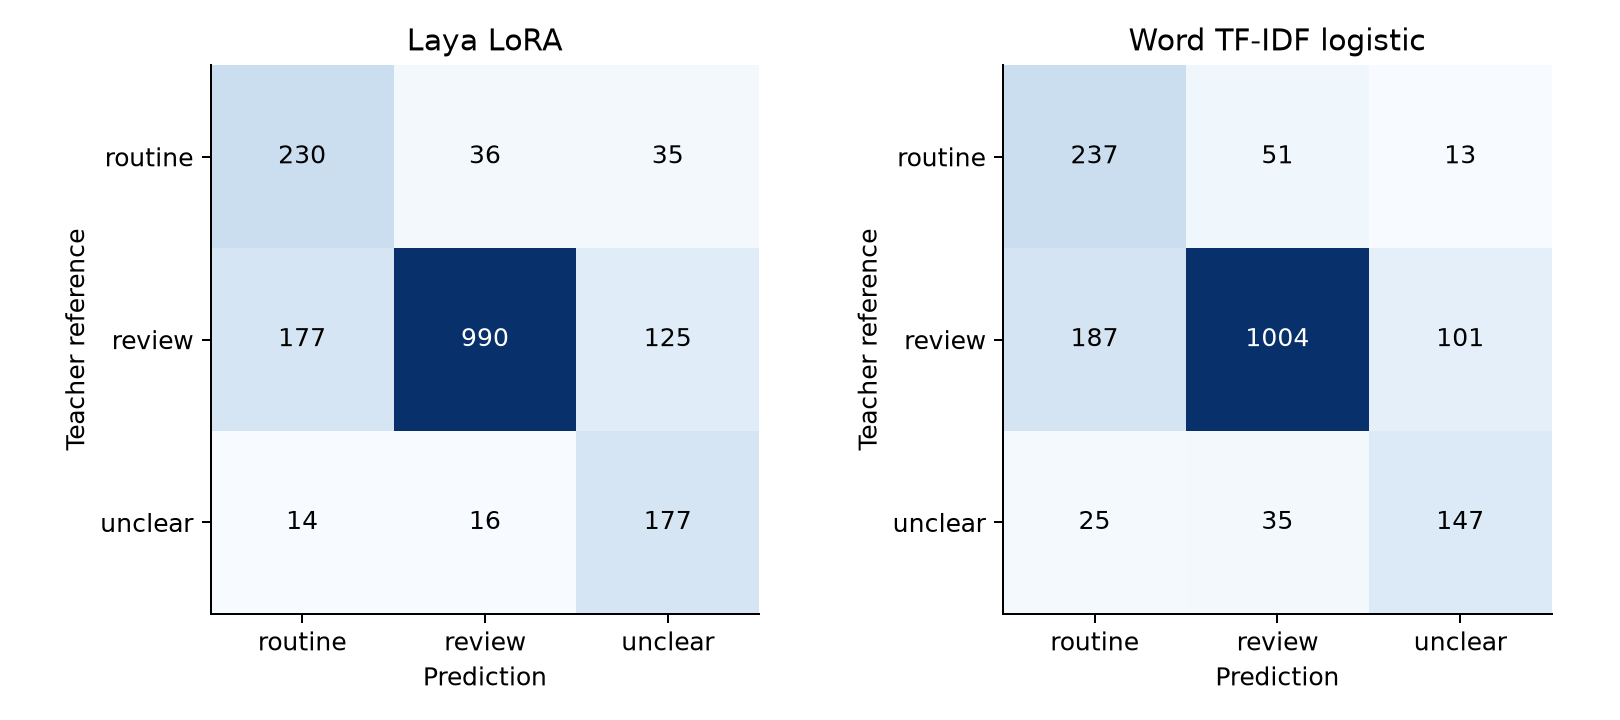
\includegraphics[width=0.95\linewidth]{confusion.png}
\caption{Primary held-out confusion matrices. Rows are teacher references and
columns are predictions; \emph{review} denotes review-worthy.}
\label{fig:confusion}
\end{figure}

\subsection{Exploratory class decomposition and routing}
Analyses in this subsection were added after viewing the test results. The unclear
class contributes approximately 68.3\% of the primary macro-F1 point difference.
Its contribution is 0.0075, versus 0.0017 for routine and 0.0018 for review-worthy;
every class-contribution interval includes zero. This decomposition clarifies
what the aggregate endpoint rewards without changing that endpoint.

Collapsing the existing predictions into discard versus review gives macro F1
0.7730 for Laya and 0.7676 for TF-IDF, with paired difference interval
$[-0.0176,0.0281]$. Among 1,499 references requiring review (review-worthy or
unclear), Laya discards 191 versus 212 while sending 28 more documents for review.
The paired required-review miss-rate difference interval also includes zero.
These derived routing results do not establish a resolved operational advantage.

\subsection{Calibrated discard policies}
Temperature scaling reduces Laya's test Brier score from 0.303 to 0.300 and ECE
from 0.049 to 0.034; TF-IDF changes from 0.313 to 0.304 and from 0.067 to 0.028
respectively. These confidence improvements do not establish a safe discard
rule. Table~\ref{tab:policies} shows that both primary systems exceed both nominal
calibration targets on test. For example, Laya's 5\% policy removes 14.72\% of
workload but misses 6.58\% of teacher review-worthy references.

\begin{table}[tbp]
\centering
\caption{Frozen calibration-selected policies on test. Target names denote
empirical calibration constraints, not achieved test bounds.}
\label{tab:policies}
\small
\begin{tabular}{@{}llrrr@{}}
\toprule
Method & Target & Workload removed & Misses & Miss rate\\
\midrule
Laya LoRA & 1\% & 5.39\% & 17 & 1.32\%\\
Laya LoRA & 5\% & 14.72\% & 85 & 6.58\%\\
Word TF-IDF/logistic & 1\% & 6.72\% & 16 & 1.24\%\\
Word TF-IDF/logistic & 5\% & 13.44\% & 65 & 5.03\%\\
\bottomrule
\end{tabular}
\end{table}

Figure~\ref{fig:policies} adds post-hoc uncertainty around the existing frozen
policies. At 1\%, Laya removes less workload than TF-IDF while the miss-rate
difference remains unresolved. At 5\%, the nominal paired miss-rate-difference
interval is unfavorable to Laya, while the workload difference remains
unresolved. Separate marginal bars are not joint confidence regions. No new
threshold was selected from these test outcomes.

\begin{figure}[tbp]
\centering
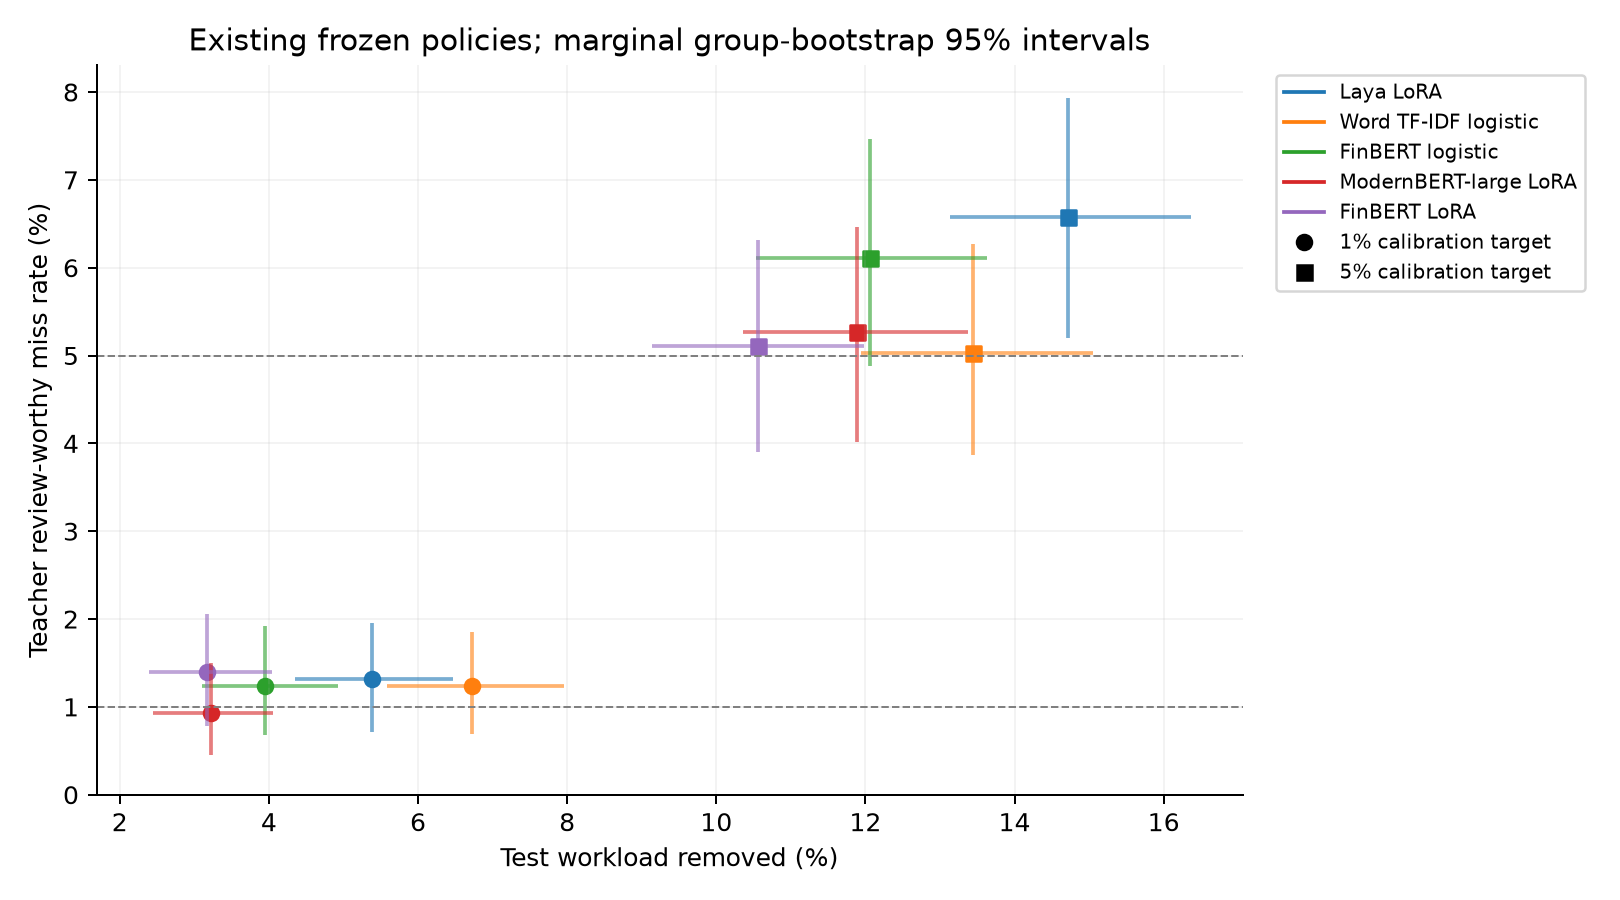
\includegraphics[width=0.95\linewidth]{diagnostic-policies.png}
\caption{Exploratory uncertainty around ten original frozen policy points.
Circles and squares denote 1\% and 5\% calibration targets. Horizontal and
vertical bars are separate marginal whole-group 95\% intervals.}
\label{fig:policies}
\end{figure}

\subsection{Adaptation, label count and contiguous context}
Matched pre-update comparisons establish supervised task learning:
Laya LoRA improves from 0.364 to 0.712 test F1, Laya head from 0.364 to 0.545,
ModernBERT LoRA from 0.096 to 0.689, and FinBERT LoRA from 0.097 to 0.642.
Their paired gain intervals are $[0.317,0.377]$, $[0.151,0.211]$,
$[0.569,0.617]$ and $[0.521,0.568]$ respectively. Pre-update controls
do not demonstrate superiority over a trained frozen-feature classifier;
Laya retains a pretrained native decision head, while the encoder alternatives
start with fresh triage classifiers.

Figure~\ref{fig:learning} reports the frozen learning curves. Laya LoRA's
1k-to-4k increment improves F1 by 0.071, with paired interval $[0.049,0.093]$.
Word TF-IDF/logistic gains 0.084 from 4k to 16k, interval $[0.061,0.109]$;
its 16k-to-25k gain is approximately 0.002, interval $[-0.013,0.016]$.
Additional labels help particular recipes, but these points do not identify
universal minimum sample requirements. Source/class allocations vary, and
recipe screening plus 1,200 selection/calibration labels are additional to
each reported training size.

\begin{figure}[tbp]
\centering
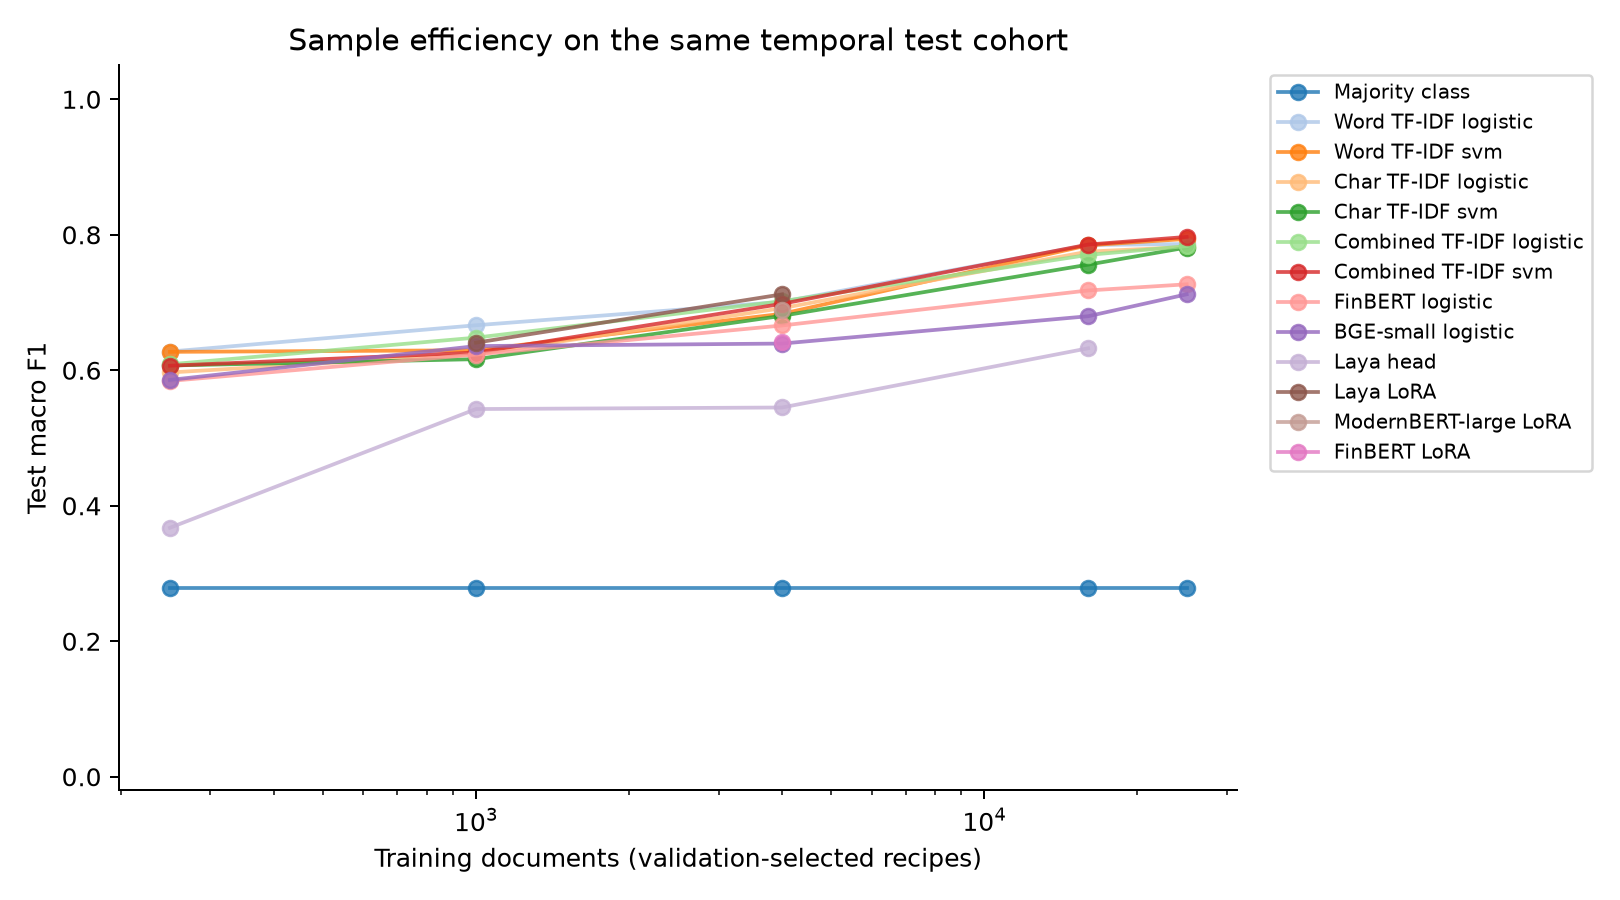
\includegraphics[width=0.97\linewidth]{learning-curves.png}
\caption{Frozen sample-efficiency comparisons on the same test cohort. The
larger lexical and head curves are supplementary; the primary trained-model
comparison remains at 4k. Exact allocations and all paired increments are
available in the evidence package.}
\label{fig:learning}
\end{figure}

The Laya head context ablation is not monotonic (Figure~\ref{fig:context}).
The 512-to-1,024-token paired F1 difference interval is $[-0.014,0.031]$;
512 to 4,096 yields $[-0.052,-0.006]$. All source tokens remain covered,
while contiguous context and pooled vote count change together. This
supplementary, uncorrected head experiment does not isolate context from
aggregation or establish a LoRA context result.

\begin{figure}[tbp]
\centering
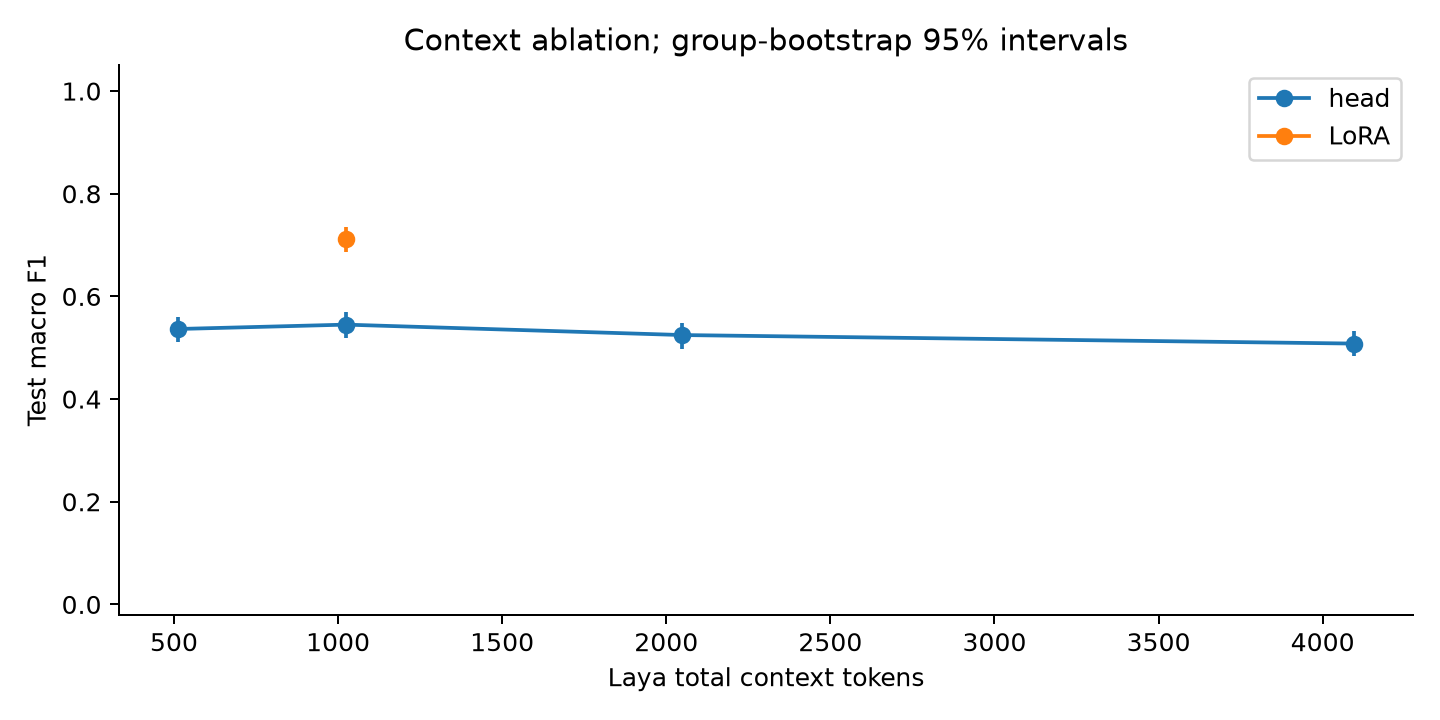
\includegraphics[width=0.92\linewidth]{context.png}
\caption{Laya context ablation under whole-document uniform pooling, with
marginal group-bootstrap 95\% intervals. The lone LoRA point is a reference,
not a LoRA context sweep.}
\label{fig:context}
\end{figure}

\subsection{Throughput and resources}
Figure~\ref{fig:throughput} shows held-out agreement against local warm throughput.
Table~\ref{tab:resources} gives neural training and accelerator memory measurements.
Laya's higher parameter-update budget, window behavior and classifier architecture
qualify any interpretation of cost as a property of decision models alone.
Cache reuse also means classifier fitting time alone understates frozen-encoder
preparation. Detailed batch throughput, feature clocks, checkpoint sizes and
parameter counts are retained with the measurements.

\begin{figure}[tbp]
\centering
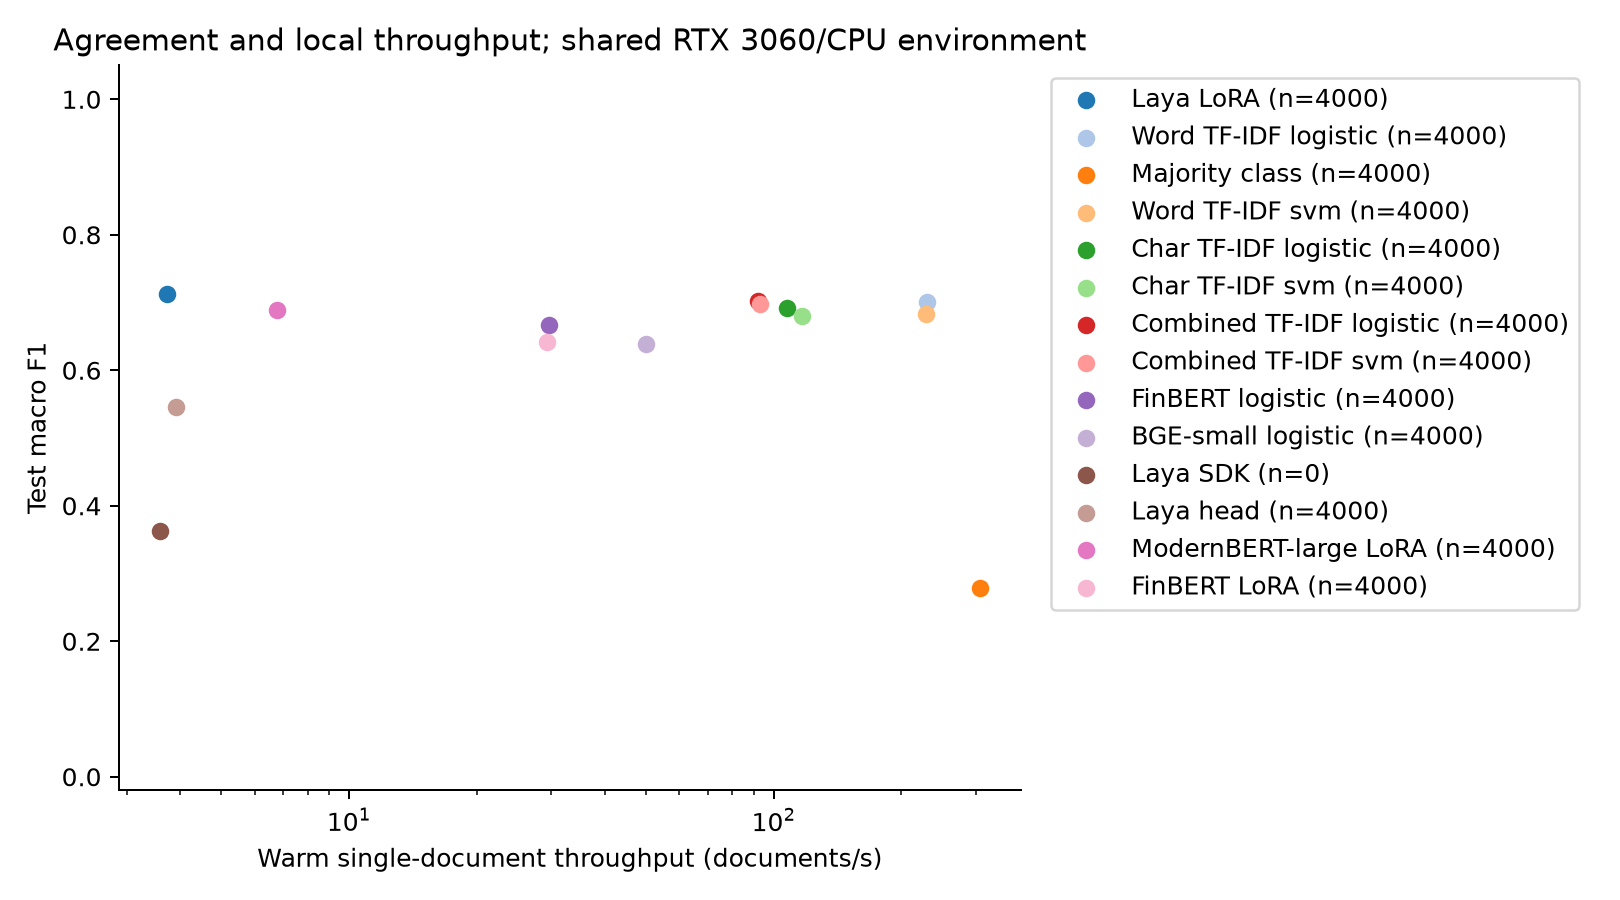
\includegraphics[width=0.97\linewidth]{throughput.png}
\caption{Held-out agreement versus warm single-document throughput in the
shared RTX 3060/CPU environment. Loading is excluded; every source window and
preprocessing are included. Different batching behavior prevents treating the
figure as a production service benchmark.}
\label{fig:throughput}
\end{figure}

\begin{table}[tbp]
\centering
\caption{Neural resource measurements. Training includes validation but excludes
startup and final calibration/resource work. Memory is peak allocated VRAM.}
\label{tab:resources}
\small
\begin{tabularx}{\linewidth}{@{}Xrrrr@{}}
\toprule
Method & Train h & Train GiB & Infer GiB & P95 ms\\
\midrule
Laya LoRA & 3.88 & 3.18 & 2.11 & 1,127.9\\
Laya head & 1.99 & 2.35 & 2.09 & 1,065.1\\
ModernBERT-large LoRA & 2.17 & 2.88 & 1.81 & 525.4\\
FinBERT LoRA & 0.54 & 0.78 & 0.52 & 117.6\\
\bottomrule
\end{tabularx}
\end{table}

\subsection{Exploratory source, length and shared-error analysis}
Figure~\ref{fig:slices} reports post-hoc source and length slices. The 6-K paired
difference has a nominal positive interval, with no multiplicity correction.
All four length-band difference intervals include zero. Cutpoints
2,695/4,589/9,835 characters come from selection quartiles, not token budgets.
Source and length are confounded. Moreover, families lacking unclear references
have an attainable fixed-three-class F1 ceiling of $2/3$ under
Equation~\ref{eq:f1}; raw family F1 values should not be compared as though their
class support were identical.

Both primary systems miss 105 teacher review-worthy documents, with 72 additional
Laya-only and 82 TF-IDF-only misses. Such overlap motivates a possible future
cascade, but does not measure its false positives, workload or computational
tradeoffs. Shared errors might also contain questionable teacher references.
Independent adjudication is needed to distinguish those cases; confidence does
not establish reference validity.

\begin{figure}[tbp]
\centering
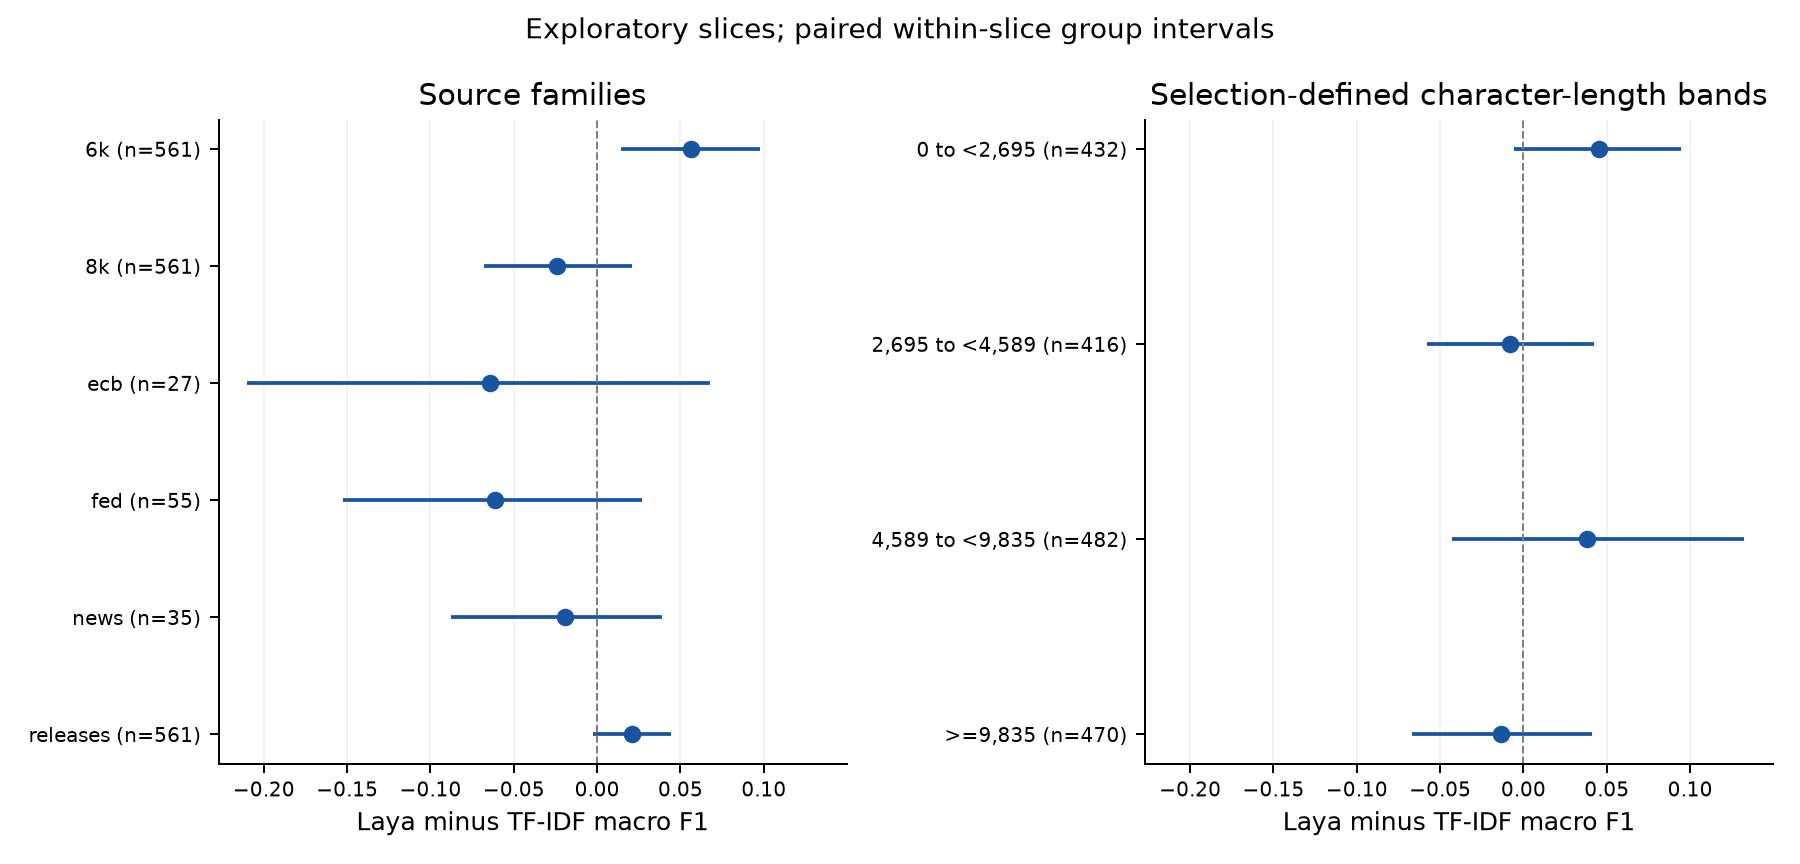
\includegraphics[width=0.97\linewidth]{diagnostic-slices.png}
\caption{Exploratory Laya-minus-TF-IDF F1 differences by source family and
selection-defined character-length band. Bars are paired within-slice
whole-group 95\% intervals, retaining three fixed labels. These uncorrected,
conditional comparisons are not causal context tests.}
\label{fig:slices}
\end{figure}

\FloatBarrier
\section{Development-only encoder extensions}
\label{sec:development}
After inspecting the original test outcomes, two additional fits examined more
FinBERT labels and a compact BGE encoder. They use only training, selection and
calibration cohorts. The 837-document selection set chooses checkpoints, and
the 363-document calibration set fits confidence and policies. Both are fitting
cohorts. Table~\ref{tab:development} must therefore not be interpreted as an
extension of the held-out leaderboard in Table~\ref{tab:main}.

All new neural fits start from pinned pretrained weights and use 512-token
context, uniform pooling, rank eight, scaling 16, adapter dropout 0.05,
unweighted cross-entropy, head/encoder learning rates $10^{-4}$ and seed 42.
Three epochs are allowed, with epoch zero eligible. Both FinBERT sizes select
epoch three; BGE selects epoch two. Architecture and classifier recipes still
differ.

\begin{table}[tbp]
\centering
\caption{Development fitting evidence, not new test results. Misses are
review-worthy references discarded out of 552; unclear discards are out of
93, and all discards out of 837.}
\label{tab:development}
\small
\setlength{\tabcolsep}{4pt}
\begin{tabularx}{\linewidth}{@{}Xrrrrr@{}}
\toprule
Method / train size & F1 & Misses & Unclear & Discards & Mean ms\\
\midrule
FinBERT LoRA / 4k & 0.6715 & 132 & 5 & 286 & 33.94\\
FinBERT LoRA / 16k & 0.7636 & 67 & 17 & 242 & 34.02\\
BGE-small LoRA / 4k & 0.6586 & 84 & 7 & 219 & 20.23\\
Frozen BGE/logistic / 4k & 0.6459 & 109 & 9 & 242 & 20.40\\
\bottomrule
\end{tabularx}
\end{table}
\FloatBarrier

\subsection{FinBERT label scaling}
The fixed-recipe 4k-to-16k comparison improves selection F1 by 0.0921 and reduces
critical misses from 132 to 67. It sends 44 more documents for review while
discarding twelve additional unclear references. Training/validation time
increases from 32.6 to 143.1 minutes, a factor of 4.38; warm inference latency
is approximately unchanged. The nested training cohorts have routine/review-worthy/
unclear counts of 1,648/1,720/632 and 5,535/7,987/2,478 respectively.

Sample count, source/class composition and optimizer steps (1,500 versus 6,000)
change together. This is promising fitting evidence for a fresh evaluation
question, not an isolated causal effect of data volume or a minimum sample
requirement. The 16k FinBERT 1\% policy still misses 1.45\% of selection
review-worthy references.

\subsection{Compact-encoder tradeoffs}
At matched 4k size, BGE LoRA has slightly lower selection F1 than FinBERT LoRA
but lower warm mean latency (20.23 versus 33.94 ms), training peak memory
(0.32 versus 0.78 GiB) and inference peak memory (0.19 versus 0.52 GiB).
Its 84 versus 132 critical misses come with 67 additional documents for review
and two additional unclear discards. Relative to frozen BGE, its small F1 gain
and 25 fewer critical misses come with 23 extra reviews. These operating points
show a resource/workload tradeoff, not operational dominance.

BGE training/validation takes 21.0 minutes and updates 149,379 parameters,
versus FinBERT's 298,755. Its matched epoch-zero selection F1 is 0.3120;
the observed gain includes learning a fresh classifier and encoder adapters.
All three matched-4k systems exceed both calibration miss targets on selection.
Different architectures, pretrained objectives and classifier recipes prevent
attributing differences solely to finance pretraining or LoRA. Neither extension
adds a 65th frozen test result, revises the core conclusion or supports an
independent generalization/significance claim. A future comparison requires
fresh held-out data.

\section{Discussion and limitations}
The held-out comparison supports retaining lexical classifiers as serious
throughput baselines for this teacher-labeled public-source task. Adaptation
learns the labeling convention, and more data helps some recipes, but the
primary F1 interval does not resolve an advantage commensurate with Laya's
much higher measured latency. Macro F1, critical misses and review workload
also capture different aspects of behavior. Favorable miss counts can reflect
more escalation rather than a strictly better decision boundary.

Reference validity is the central limitation. Training and test labels come
from the same teacher, so the experiment measures imitation on new documents,
not analyst-validated materiality. The unclear class, thin filing cover sheets
and possible reference disagreements make independent adjudication especially
relevant. The test set is dominated by SEC content and contains official
announcements rather than broad contemporary journalism. Historical snapshot
revision, possible pretraining exposure and unrecognized duplicate relationships
remain threats to stronger generalization claims.

One trained seed and conditional bootstrap intervals do not characterize
optimization instability. Recipe comparisons are bounded, not exhaustive:
there is no measured frontier generative-model comparator, full adaptation
sweep, or reinforcement-learning/RLCD adaptation result. Supplementary
contrasts and post-hoc slices are uncorrected for multiplicity. The subsequent
encoder fits use reused development cohorts after test inspection, so their
scores can guide a new experiment but cannot identify a new test-set winner.
Hardware timings likewise do not establish energy, deployment or cloud costs.
No systematic-strategy profitability is evaluated.

\section{Conclusion}
In the frozen equal-data comparison, adapted Laya attains a small F1 point
advantage over word TF-IDF/logistic regression that remains unresolved under
paired group-bootstrap uncertainty, with approximately 59-fold higher local
warm mean latency. Supervised adaptation and additional labels improve
particular recipes; longer head context is not monotonically beneficial, and
calibration-selected miss targets fail to transfer as test guarantees.
Development-only FinBERT scaling and compact BGE adaptation provide useful
resource and label-efficiency questions for a fresh study. Stronger operational
claims require independently reviewed references and a new representative
held-out cohort, with methods and policies selected before evaluation.

\section*{Code, evidence and reproducibility}
The public repository provides all 64 frozen comparisons, ordered logits and
teacher references, fixed decisions, full metric/statistics tables, recorded
resources and independent audit receipts. Both development fits have separate
probability, cohort, history and verification bundles. The versioned evidence
package is available at
\href{https://github.com/LuccaPereiraMartins/systematic-trading/tree/431d1e40a6f3b567529c5b5e986247ea706e5c62/decision_models/reports/core-v1}{the study repository (commit \texttt{431d1e4})}.
The command \texttt{python decision\_models/reports/core-v1/verify.py}
replays the published arithmetic on CPU without model weights, source bodies
or API calls. Exact training/inference replay additionally requires the
preserved local corpus/checkpoints, original directory relationships and pinned
source/dependency bytes. A fresh collection or Git clone alone cannot reconstruct
the exact historical text. Source attribution and transfer conditions are
documented in the repository. The original freeze, ownership and held-out
results remain preserved.

\FloatBarrier
\begin{thebibliography}{10}
\small
\raggedright
\setlength{\itemsep}{2pt}
\setlength{\parskip}{0pt}
\bibitem{wang}
Sida Wang and Christopher D. Manning.
Baselines and bigrams: Simple, good sentiment and topic classification.
In \emph{Proceedings of the 50th Annual Meeting of the Association for
Computational Linguistics (Volume 2: Short Papers)}, pp.\ 90--94, 2012.
\url{https://aclanthology.org/P12-2018/}.

\bibitem{finbert}
Dogu Araci.
FinBERT: Financial sentiment analysis with pre-trained language models.
2019. \href{https://arxiv.org/abs/1908.10063}{arXiv:1908.10063}.

\bibitem{modernbert}
Benjamin Warner et al.
Smarter, better, faster, longer: A modern bidirectional encoder for fast,
memory efficient, and long context finetuning and inference.
2024. \href{https://arxiv.org/abs/2412.13663}{arXiv:2412.13663}.

\bibitem{bge}
Beijing Academy of Artificial Intelligence.
\emph{BAAI/bge-small-en-v1.5 model card}.
\url{https://huggingface.co/BAAI/bge-small-en-v1.5}.
Checkpoint revision \texttt{5c38ec7c405e}; accessed October 2026.

\bibitem{laya}
ConvAI Innovations.
\emph{Laya model card}, pinned English root checkpoint.
\url{https://huggingface.co/convaiinnovations/laya}.
Checkpoint revision \texttt{55cf4c4ebb4e}; accessed October 2026.

\bibitem{lora}
Edward J. Hu, Yelong Shen, Phillip Wallis, Zeyuan Allen-Zhu, Yuanzhi Li,
Shean Wang, Lu Wang, and Weizhu Chen.
LoRA: Low-rank adaptation of large language models.
2021. \href{https://arxiv.org/abs/2106.09685}{arXiv:2106.09685}.

\bibitem{gneiting}
Tilmann Gneiting and Adrian E. Raftery.
Strictly proper scoring rules, prediction, and estimation.
\emph{Journal of the American Statistical Association}, 102(477):359--378,
2007. \href{https://doi.org/10.1198/016214506000001437}{doi:10.1198/016214506000001437}.

\bibitem{guo}
Chuan Guo, Geoff Pleiss, Yu Sun, and Kilian Q. Weinberger.
On calibration of modern neural networks.
In \emph{Proceedings of the 34th International Conference on Machine Learning},
2017. \href{https://arxiv.org/abs/1706.04599}{arXiv:1706.04599}.

\bibitem{annotation}
Nicholas Pangakis, Samuel Wolken, and Neil Fasching.
Automated annotation with generative AI requires validation.
2023. \href{https://arxiv.org/abs/2306.00176}{arXiv:2306.00176}.
\end{thebibliography}
\end{document}
